\documentclass[mathserif]{beamer}

\mode<presentation> {
	\usetheme{PaloAlto}
	\usecolortheme{whale}
}

\usepackage{xeCJK}
\setCJKmainfont{STKaiti}

\usepackage{algorithm}
\usepackage{algorithmic}
\usepackage{graphicx}
\usepackage{booktabs}
\usepackage{fontspec}
\usepackage{xunicode}
\usepackage{xltxtra}
\usepackage{longtable}

\usepackage{amsmath,amssymb}

%\usepackage{syntonly}
%\syntaxonly

\setbeamercovered{transparent}
%\logo{
\includegraphics[height=1.58cm]{./logo.jpg}}

\title[Venti]{Venti: a new approach to archival storage\thanks{powered by \XeLaTeX}}

\author{Presented By: 陈子旸}
\institute[FDU]
{
	Fudan University\\
	\medskip
	\textit{13307130148@fudan.edu.cn}
}
\date{\today}

\begin{document}
\newtheorem{property}[theorem]{\textsc{Property}}
\newtheorem{defination}[theorem]{\textsc{Defination}}
\newtheorem{theore}[theorem]{\textsc{Theorem}}
\newtheorem{lemm}[theorem]{\textsc{Lemma}}

\begin{frame}
\titlepage
\end{frame}

\AtBeginSection{
	\begin{frame}
	\frametitle{Outline}
	\tableofcontents[currentsection, hideothersubsections]
	\end{frame}
}

\section{Overview}\label{overview}

\subsection{Abstract}\label{abstract}

\begin{frame}{Abstract}

\begin{itemize}
\itemsep1pt\parskip0pt\parsep0pt
\item
  Describes a pedestrian population trend estimation method using
  location data of smartphone users.
\item
  Intended to be an alternative to traffic censuses using tally
  counters.
\item
  Using smartphone users' location data accumulated on Yahoo! Japan.
\item
  Tackles the problem of data shortage when a target area is a small
  region by using a Gaussian kernel.
\end{itemize}

\end{frame}

\subsection{Background}\label{background}

\begin{frame}{Background}

\begin{itemize}
\itemsep1pt\parskip0pt\parsep0pt
\item
  Knowing the number of pedestrians in a time or place can be an
  essential data source for market research.
\item
  Triditional method: Traffic censuses using tally counters are still
  commonly used.

  \begin{enumerate}
  \def\labelenumi{\arabic{enumi})}
  \itemsep1pt\parskip0pt\parsep0pt
  \item
    Requires many survey crews and much time.
  \item
    Temporal and spatial limitation.
  \end{enumerate}
\item
  Location-based services (LBSs) are widely used by smartphone users
\item
  two problems remain

  \begin{enumerate}
  \def\labelenumi{\arabic{enumi})}
  \itemsep1pt\parskip0pt\parsep0pt
  \item
    How to pick out only pedestrians.
  \item
    How to set the research area and period.
  \end{enumerate}
\end{itemize}

\end{frame}

\section{Data Set}\label{data-set}

\begin{frame}{Data Set}

\begin{itemize}
\itemsep1pt\parskip0pt\parsep0pt
\item
  The location data are provided by smartphone users through services of
  Yahoo! Japan, contains:

  \begin{itemize}
  \itemsep1pt\parskip0pt\parsep0pt
  \item
    Latitude
  \item
    Longitude
  \item
    Horizontal accuracy
  \item
    Time stamp (at a second rate)
  \item
    Anonymized user ID (changes after 24 hours)
  \end{itemize}
\end{itemize}

\end{frame}

\begin{frame}{Data Set}

\begin{figure}
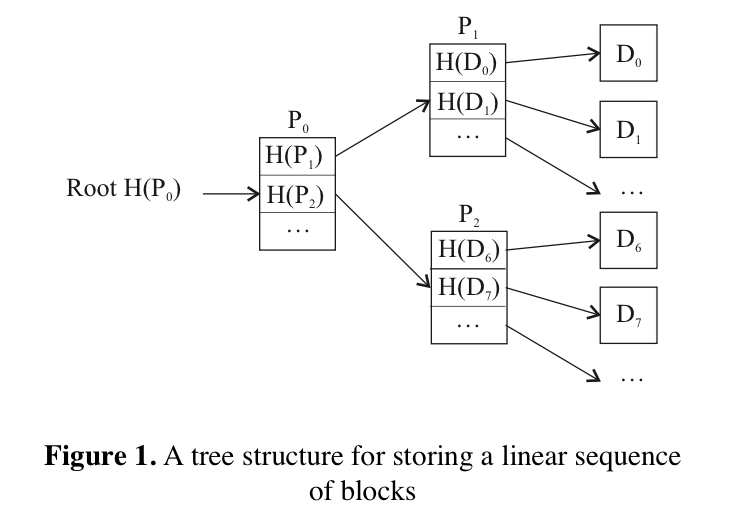
\includegraphics[width = 10cm]{pic1.png}\\
Table: Examples of the location data
\end{figure}

\end{frame}

\begin{frame}{Data Set}

\begin{figure}
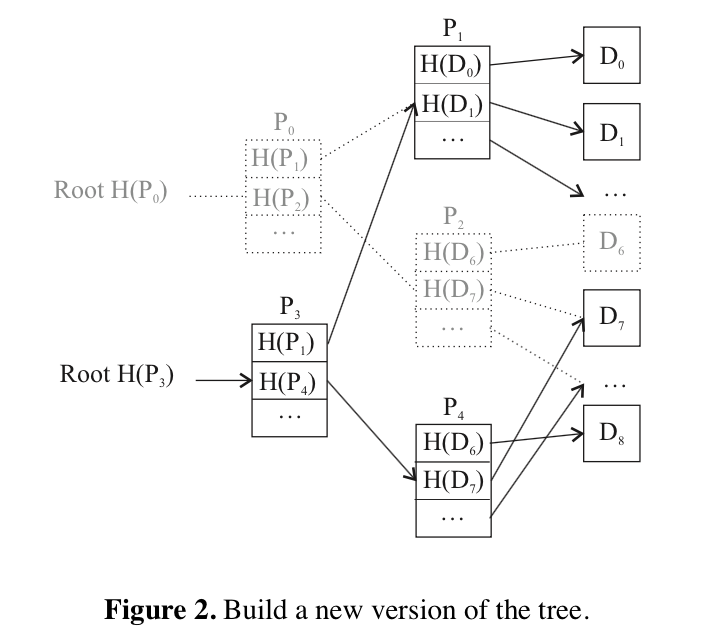
\includegraphics[height = 4cm]{pic2.png}
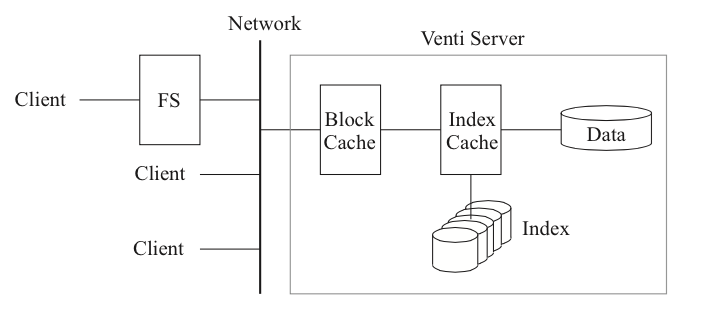
\includegraphics[height = 4cm]{pic3.png}
\end{figure}

\end{frame}

\section{Method}\label{method}

\subsection{Simple approach}\label{simple-approach}

\begin{frame}{A simple approach}

\begin{itemize}
\itemsep1pt\parskip0pt\parsep0pt
\item
  Assumes that the number of records in an area is proportional to the
  people present in the area.

  \begin{itemize}
  \itemsep1pt\parskip0pt\parsep0pt
  \item
    Determine target areas(polygonal) and target days
  \item
    Number of records existing in the area hourly is counted and then
    multiplied by a proper factor.
  \item
    The date has errors more than 300 meters are eliminated.
  \end{itemize}
\end{itemize}

\end{frame}

\begin{frame}{A simple approach}

\begin{figure}
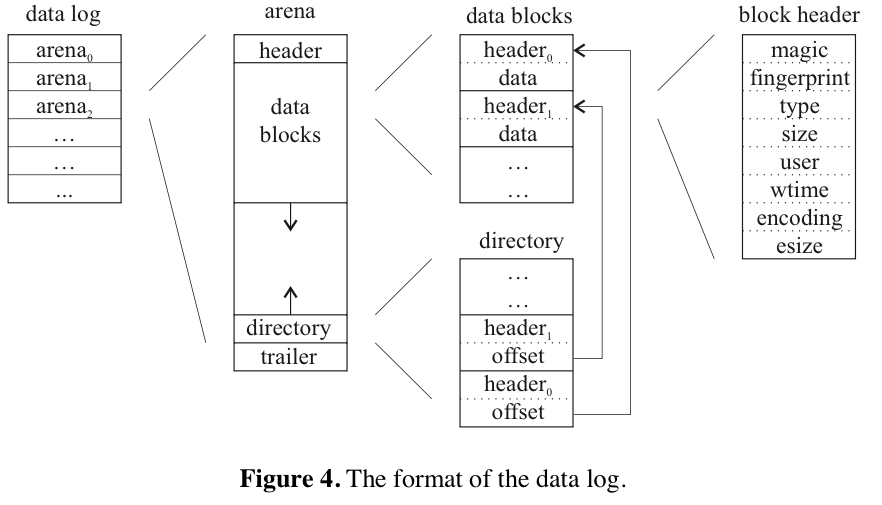
\includegraphics[height = 4cm]{pic4.png}
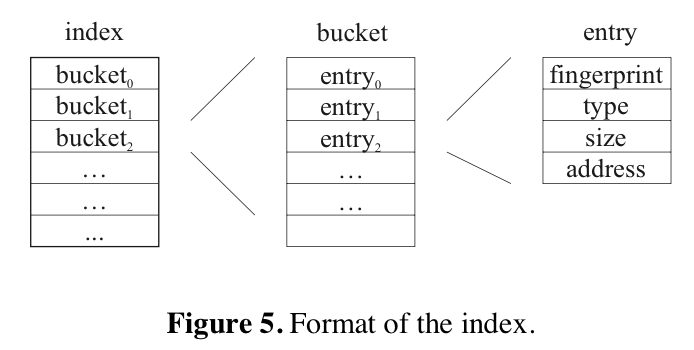
\includegraphics[height = 4cm]{pic5.png}
\end{figure}

\end{frame}

\begin{frame}{Limitation of the simple approach}

\begin{itemize}
\itemsep1pt\parskip0pt\parsep0pt
\item
  Non-pedestrian records

  \begin{itemize}
  \itemsep1pt\parskip0pt\parsep0pt
  \item
    stationary users (e.g.~in offices)
  \item
    passing users (e.g.~on trains)
  \end{itemize}
\item
  Time continuous estimation
\item
  Sparsity with the smallness of target areas.
\end{itemize}

\end{frame}

\subsection{Improvement method}\label{improvement-method}

\begin{frame}{Eliminating non-pedestrian data}

\begin{figure}
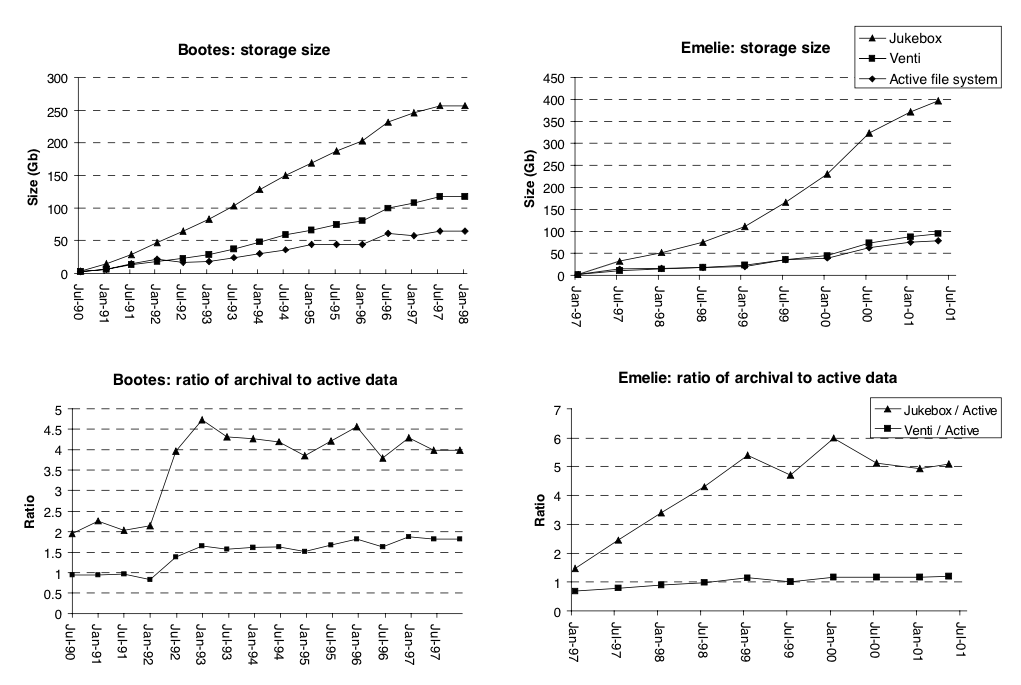
\includegraphics[height = 4cm]{pic6.png} 
\end{figure}

\begin{itemize}
\itemsep1pt\parskip0pt\parsep0pt
\item
  Data are extracted user-by-user(by user id).
\item
  Approximate mean velocity is estimated an hour before or after a
  person visits the target area.
\item
  The records where velocities both before and after are high or near
  zero are eliminated.
\end{itemize}

\end{frame}

\begin{frame}{Realizing time-continuous estimation}

\begin{itemize}
\itemsep1pt\parskip0pt\parsep0pt
\item
  Use Poisson distribution to represent counting data
  \[p(m|\lambda) = \frac{1}{m!}\lambda^{m}e^{-\lambda}\]
\item
  Consider \(\lambda\) as a function of time \(\lambda(t)\)
  \[p(m|\lambda(\cdot)) =  \frac{1}{m!}E[m]^{m}e^{-E[m]}\]
  \[E[m] = \int_{t_1}^{t_2}\lambda(t)\mathrm{d}t\]
\end{itemize}

\end{frame}

\begin{frame}{Realizing time-continuous estimation}

\begin{itemize}
\itemsep1pt\parskip0pt\parsep0pt
\item
  Decomposed \(\lambda(t)\) into \(f(t)\) and \(\lambda_0\)
  \[\lambda_0 = \int_0^T \lambda(t) \mathrm{d} t\;\;\;\;\; \lambda(t) = \lambda_0 f(t) \;\;\;\; \int_0^T f(t) \mathrm{d}t = 1\]
\item
  \(f(t)\) is estimated using Gaussian kernel density estimation
  \[f(t) = \frac{1}{h_t n} \sum_{i=1}^n k(\frac{t-t_i}{h_t})\;\;\;\;\;k(t) = \frac{1}{ \sqrt{2\pi} }e^{-\frac{1}{2}t^2}\]
\end{itemize}

\end{frame}

\begin{frame}{Realizing time-continuous estimation}

\begin{figure}
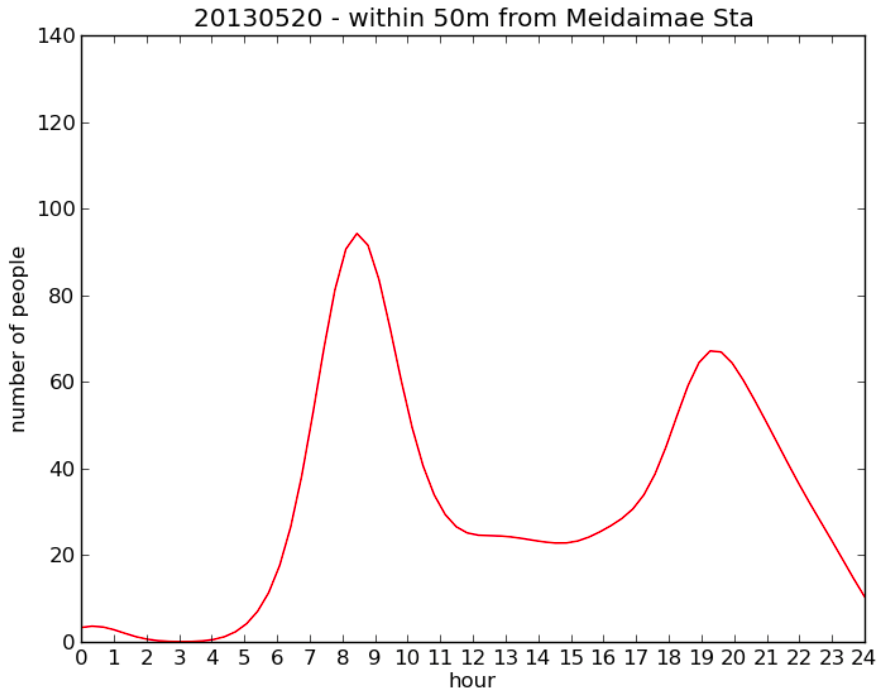
\includegraphics[width = 8cm]{pic7.png}
\end{figure}

\end{frame}

\begin{frame}{Dealing with data sparsity in space}

\begin{itemize}
\itemsep1pt\parskip0pt\parsep0pt
\item
  Data's weight \(w_i = 1\) if the data are in the target area
\item
  If the data are near the target area
  \[w_i = \frac{1}{ \sqrt{2\pi} }e^{-\frac{1}{2}(d/h_d)^2}\]
\item
  d is distance between data point and target area centroid
\item
  \(f(t)\) changed into
  \[f(t) = \frac{1}{h_t\sum w_i}\sum_{i=1}^{n}w_i k(\frac{t-t_i}{h_t})\]
\end{itemize}

\end{frame}

\begin{frame}{Parameter selection}

\begin{itemize}
\itemsep1pt\parskip0pt\parsep0pt
\item
  Traffic censuses using tally counters were conducted for this
  research.
\item
  The parameters to be determined are \(K\), means how many pedestrians
  are represented by a single data point.
  \[\hat{K_p}=\frac{M_p}{(\sum_{i=1}^n w_i)(\int_{t_1}^{t_2}f(t)\mathrm{d}t)}\]
\item
  \(t_1\) and \(t_2\) are the census start and end times
\item
  \(M_p\) is total pedestrian number according to traffic census data of
  the day.
\end{itemize}

\end{frame}

\section{Experiment}\label{experiment}

\subsection{Reference data}\label{reference-data}

\begin{frame}{Reference data}

\begin{itemize}
\itemsep1pt\parskip0pt\parsep0pt
\item
  Traffic censuses using tally counters were conducted in five areas on
  11 days in Japan in September 2013

  \begin{figure}
  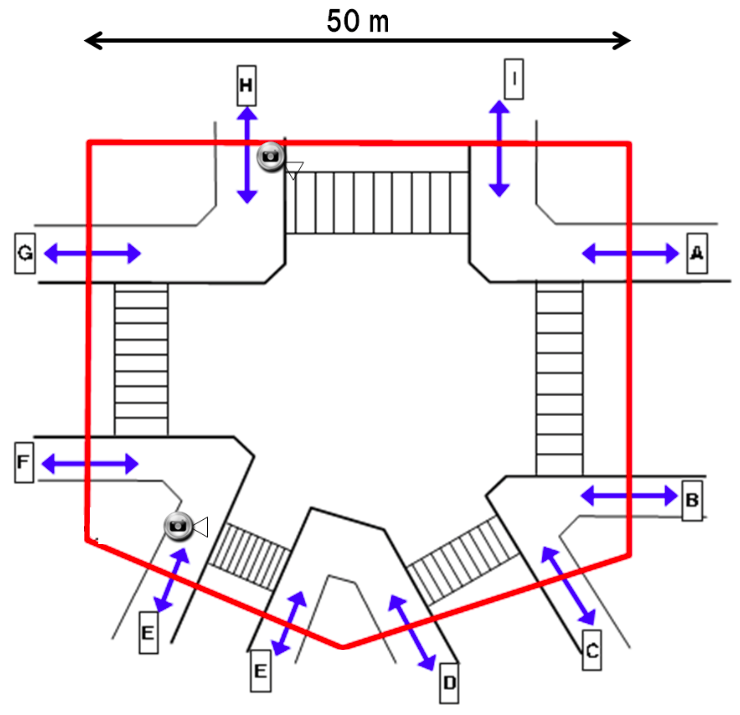
\includegraphics[height = 4cm]{pic8.png}
  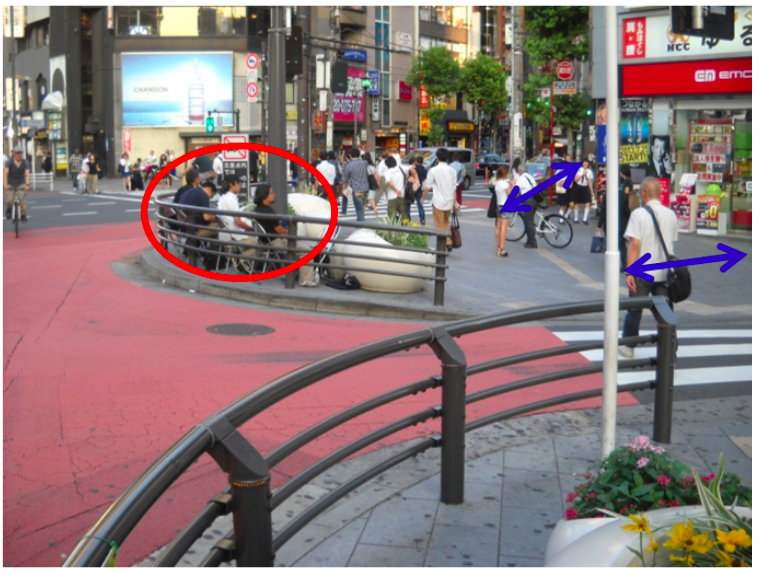
\includegraphics[height = 4cm]{pic9.png}
  \end{figure}
\end{itemize}

\end{frame}

\begin{frame}{Reference data}

\begin{figure}
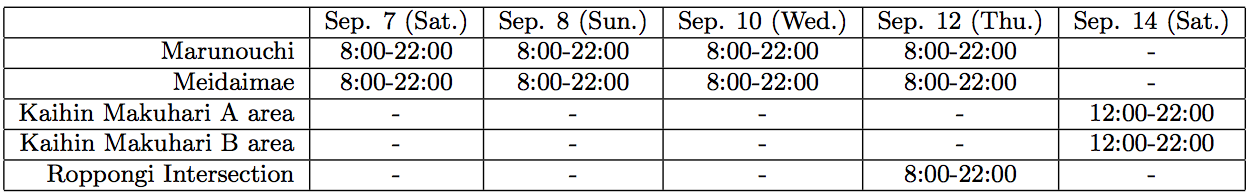
\includegraphics[width = 10cm]{pic10.png}\\
Table: Date and time of traffic census using tally counters.\\
All censuses were conducted in 2013.
\end{figure}

\end{frame}

\begin{frame}{Reference data}

\begin{figure}
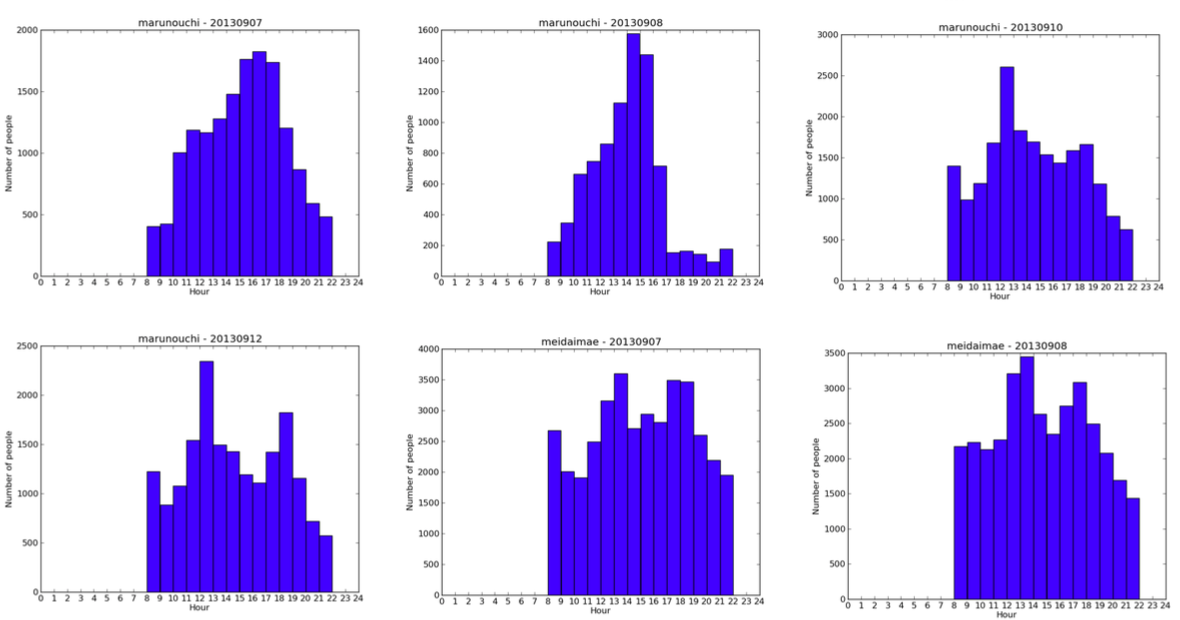
\includegraphics[width = 9cm]{pic11.png}\\
Reference data manually obtained by \\
traffic census using tally counters
\end{figure}

\end{frame}

\begin{frame}{Reference data}

\begin{figure}
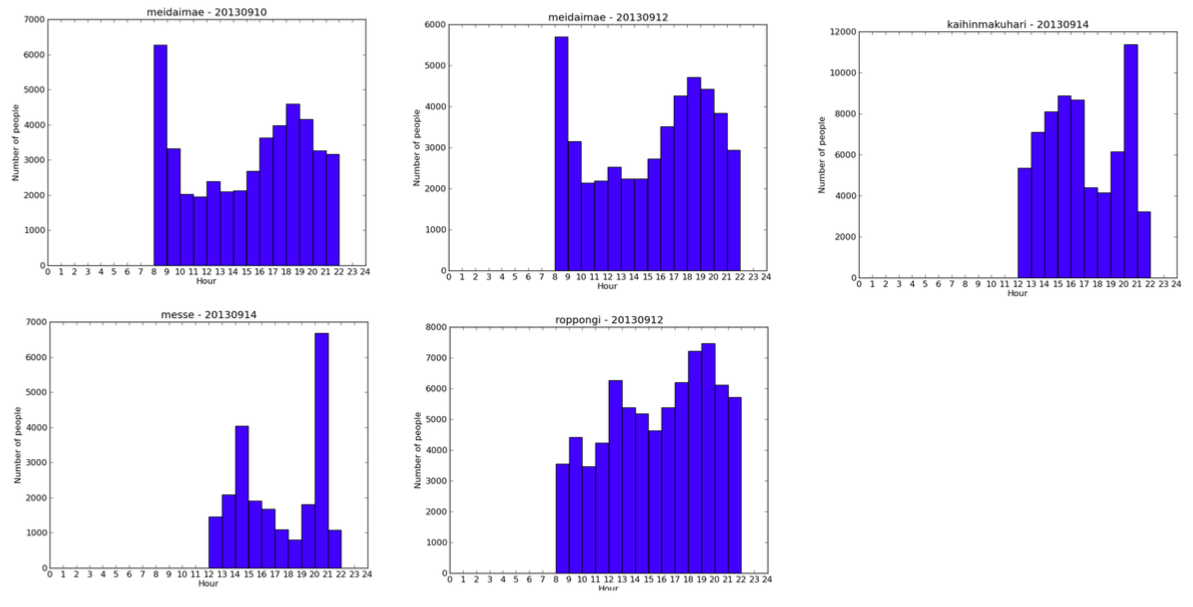
\includegraphics[width = 9cm]{pic12.png}\\
Reference data manually obtained by \\
traffic census using tally counters
\end{figure}

\end{frame}

\subsection{Evaluation metrics}\label{evaluation-metrics}

\begin{frame}{Evaluation metrics}

\begin{enumerate}
\def\labelenumi{\arabic{enumi}.}
\itemsep1pt\parskip0pt\parsep0pt
\item
  Mean squared error of hourly estimation
  \[metric\; 1 = \frac{1}{t_2-t_1}\sum_{t=t_1}^{t_2-1}(\hat{m_t}-m_t)^2\]
\item
  Absolute error of peak time
  \[metric\; 2 = |arg_t\, max(\hat{m_t}) - arg_t\, max(m_t)|\]
\item
  Absolute error of daily total number
  \[metric\; 3 = |\sum_{t=t_1}^{t_2}\hat{m_t}-\sum_{t=t_1}^{t_2}m_t|\]
\end{enumerate}

\end{frame}

\subsection{Comparative approach}\label{comparative-approach}

\begin{frame}{Comparative approach}

\begin{itemize}
\itemsep1pt\parskip0pt\parsep0pt
\item
  \textbf{Approach 1} is the simple approach. This is a method for
  counting the number of location data in a target area and hour and
  multiplying K.
\item
  \textbf{Approach 2} is almost the same as the proposed approach using
  time continuous method and data supplement using a spatial kernel
  approach, but a data elimination step is not applied.
\end{itemize}

\end{frame}

\subsection{Result}\label{result}

\begin{frame}{Result}

\begin{figure}
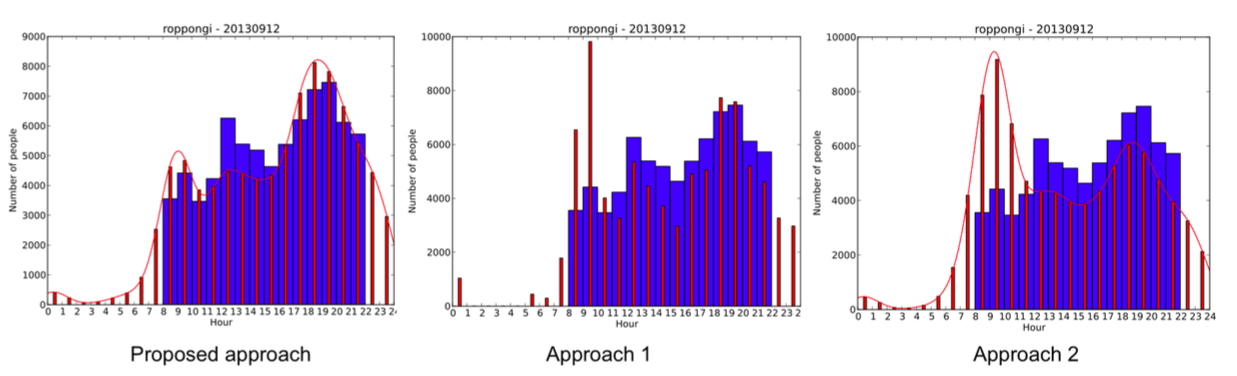
\includegraphics[width = 9cm]{pic13.png}\\
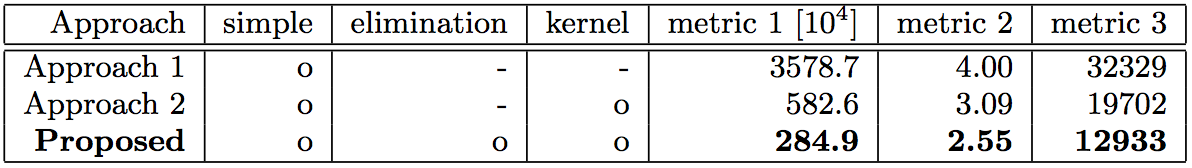
\includegraphics[width = 9cm]{pic14.png}
\end{figure}

\end{frame}

\begin{frame}{Result}

\begin{figure}
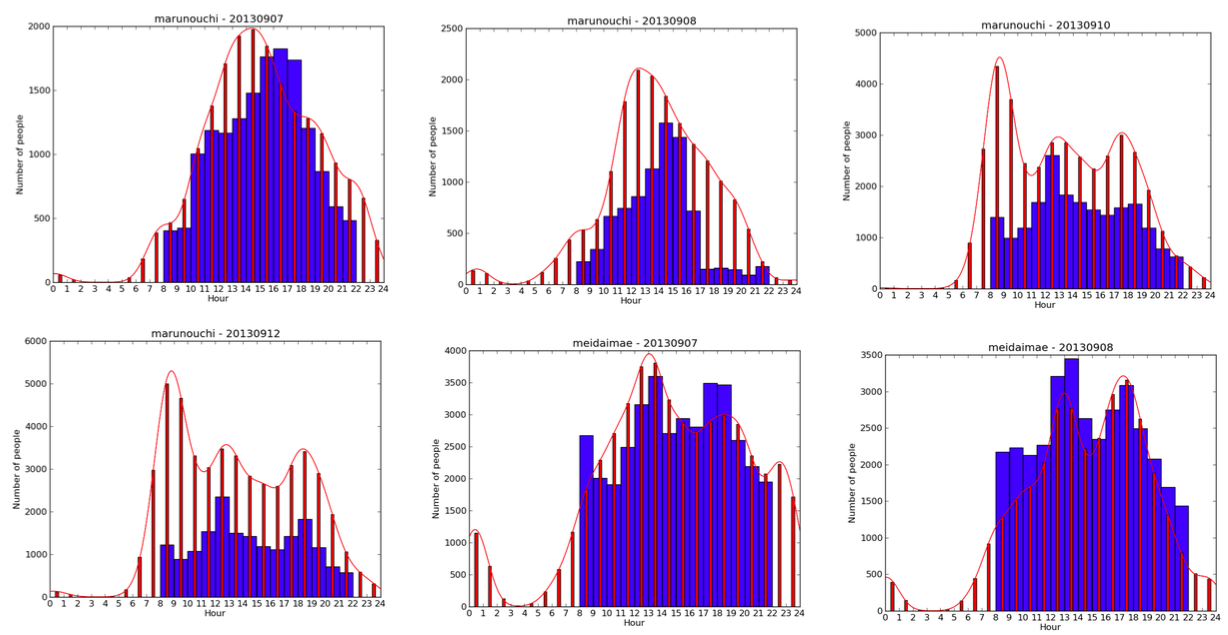
\includegraphics[width = 9cm]{pic15.png}
\end{figure}

\end{frame}

\begin{frame}{Result}

\begin{figure}
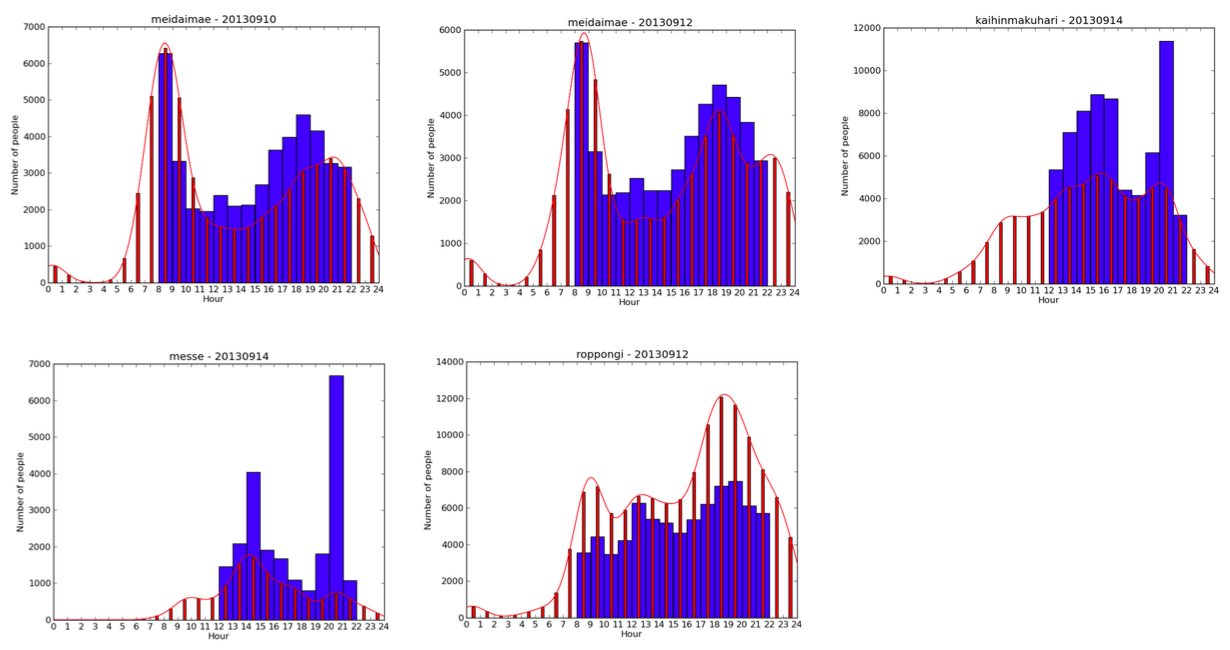
\includegraphics[width = 9cm]{pic16.png}
\end{figure}

\end{frame}

\section{Conclusion}\label{conclusion}

\begin{frame}{Conclusion}

\begin{itemize}
\itemsep1pt\parskip0pt\parsep0pt
\item
  Location data from smartphone applications were studied for monitoring
  the number of pedestrians.
\item
  Intended to be an alternative to traffic censuses using tally
  counters.
\item
  Has advantages in the cost and flexibility compared to manual censuses
\end{itemize}

\end{frame}

\begin{frame}{Conclusion}

\begin{itemize}
\itemsep1pt\parskip0pt\parsep0pt
\item
  Assume that the number of location data in an area is proportional to
  the population volume
\item
  To estimate numbers of only pedestrians
\item
  Deals with temporal and spatial sparsity of data by introducing
  non-homogeneous Poisson processes and Gaussian kernels.
\end{itemize}

\end{frame}


\AtBeginSection{}

\section[Q\&{}A]{}
\begin{frame}{Q\&{}A}
\begin{center}
  \color{blue}\huge{Any Questions?}
\end{center}
\end{frame}

\section[End]{}
\begin{frame}{End}
\begin{center}
  \color{blue}\huge{Thanks For Attention!}
\end{center}
\end{frame}

\end{document}

